%-----------------------------------------------------------------------------%
%                                                                             %
%    K A P I T E L   1                                                        %
%                                                                             %
%-----------------------------------------------------------------------------%

\chapter{Introduction}\label{c1}
This introduction guides the reader to the aim of the master's thesis. Beginning
with a motivation on humanoid robots a general problem statement is derived. Thereupon,
two approaches are presented that are pursuing different ideas of how to solve
this problem. Building upon these methods, the aim and specific objectives of the
thesis are defined. Lastly, a brief overview of the thesis structure is provided.

\section{Motivation}
\paragraph{Why Robots}
Robotics research is highly motivated by the idea of creating machines with the ability to autonomously explore and interact with complex and dynamic environments. These intelligent agents can act in surroundings that are either inaccessible or dangerous to humans or support us in everyday life tasks.
\paragraph{Why Legged Robots} 
\paragraph{Why Humanoids}
Nature often plays a crucial rule and serves as source of inspiration in the design process of such systems. This is especially true for the research field of humanoid robots, which deals with robots that are generally inspired by human capabilities and share similar kinematics, sensing and behavior. Many of the objects that we interact with on a daily basis, are tailored to human form and human behavior, e.g. doors, stairs or tools. This is equally true for the environments that we move in. Humans make use of their legs to climb stairs, lean towards difficult postures or traverse rough terrain. \cite[Ch.\ 67]{siciliano2016springer}. 
\paragraph{Vision: Exploiting Natural Dynamics}
We perform all these tasks seemingly effortless. But compared to current robots, the dynamic capabilities of humans and animals are still outstanding in terms of versatility, speed, efficiency and robustness \cite{hutter2012starleth}. In order to further close the gap between robots and their natural counterparts, current research is driving towards exploiting the natural dynamics of robots. This implies mutually dependent changes about how we think about the robots design \cite{pratt2004series} on the one hand and about ways of controlling them on the other hand, in order to move in a more dynamic, efficient and natural way \cite{collins2005efficient, haddadin2012optimal, pratt2000exploiting}.

\paragraph{Problem: Challenges in Legged Locomotion}
Legged locomotion is a challenging task since there is an ongoing need to avoid falling down, especially in contrast to wheeled robots \cite{raibert1986legged}. While some humanoids are able to perform statically stable gaits, bipedal walking mostly introduces a new level of complexity in terms of \textit{dynamic} balancing.\cite[Ch.\ 67]{siciliano2016springer}. 

The difficulty of creating bipedal walking has several causes. The first difficulty is due to the mechanism complexity, i.e.dealing with high-dimensional degrees of freedom, leading to potentially expensive computations. Secondly, legged locomotion is subject to different contact and impact collisions, resulting in multi-phase models and hence hybrid dynamics. Finally, bipeds face the problem of effective underactuation, further restricting the applicable control approaches \cite[Ch.\ 1]{westervelt2018feedback}.

\textit{Dynamic} bipedal locomotion adds additional complexity to this problem. A central characteristic of walking dynamically is that the center of mass (COM) partially leaves the biped's support polygon. Furthermore there is the need of generating feasible, controllable limit cycles. When considering running motions, difficulties are faced regarding the conservation of angular momentum, which implies restrictions on the controllability during flight phases \cite[Ch.\ 1]{westervelt2018feedback}. 


\section{Related Work}
There are existing numerous ways to generate feasible motion plans for robotic systems. Common approaches are relying on simplified dynamic models, while recent ones make use of numerical optimization for generating motion plans. 

\subsection{Traditional Legged Locomotion Planning}
Previously we have already seen, why locomotion synthesis for legged robots is a challenging problem. Solving this global problem typically is approached by splitting it up into successive subproblems that are solved sequentially: (i) Contact planner, (ii) Centroidal pattern generator, (iii) Whole-body motion generator (\cref{img:traditional_locomotion_planner}) \cite{carpentier2017multi}. 
\begin{figure}[h!]
\centering	
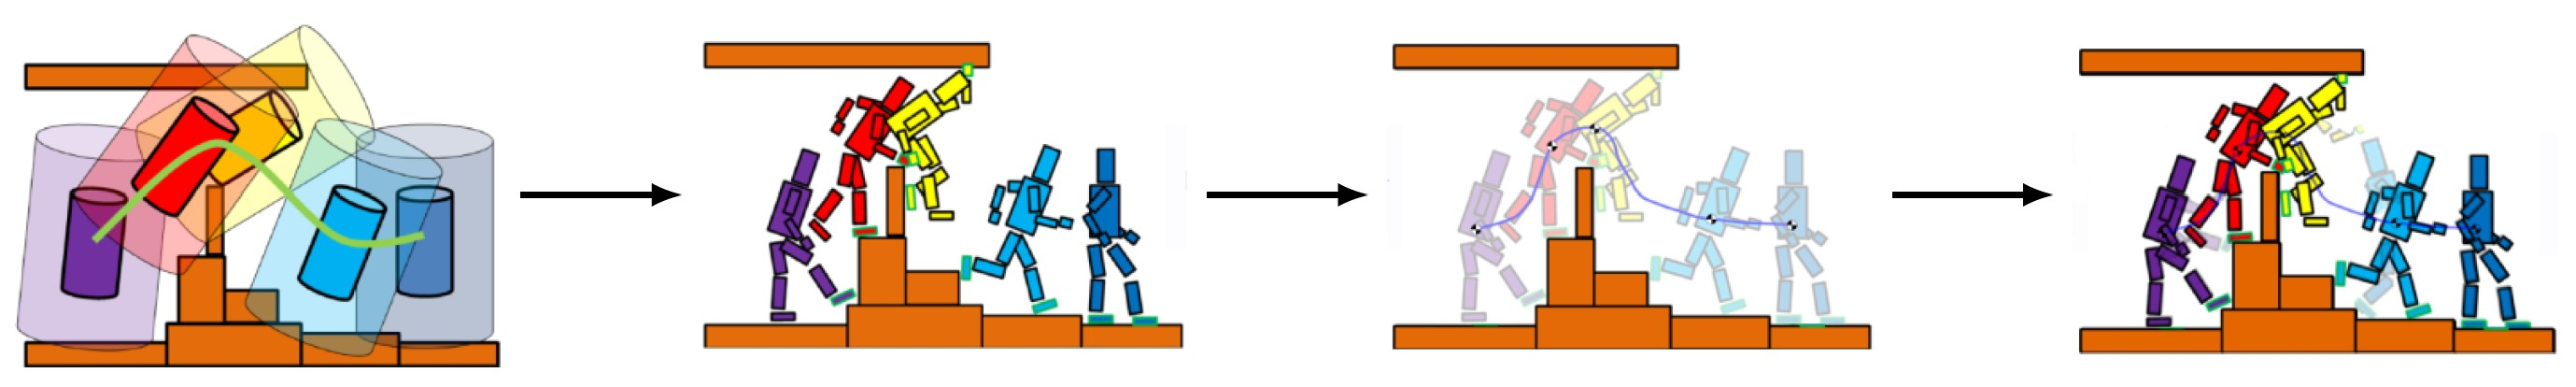
\includegraphics[width=1\textwidth]{img/traditional_locomotion_planner.jpg}
\caption{Tradional Legged Locomotion Planning \cite{giraud2020motion}.}
\label{img:traditional_locomotion_planner}
\end{figure}  
The first stage of traditional legged locomotion planning is a contact planner that selects appropriate foothold position and step timings. In other words, this component predefines \textit{where} and \textit{when} external forces can act on the system. 
Once these force locations have been predetermined, the goal is to generate a body motion, i.e. a \gls{CoM} and end-effector trajectories, which can be created with the available forces. A common approach is to model the robot as a \gls{LIP} and find a motion where the \gls{CoP} remains inside the \gls{SP}. The \gls{LIP} can be solved analytically and efficiently and consequently has been used in a variety of approaches \cite{kajita2003biped, kalakrishnan2010fast, winkler2015planning, bellicoso2017dynamic}. 
From the contact sequence and the centroidal trajectory, a dynamic-physical whole-body trajectory has to be found. This often is done by solving the \gls{IK} \cite{espiau1992new} or operational-space \gls{ID} \cite{khatib1987unified} of the system and produces appropriate joint positions or torques, respectively that can be applied to a physical system.

This approach is beneficial in terms of computation time but comes at the cost of limited motion complexity and energy efficiency. 
The first limitation comes from the underlying assumptions of the \gls{LIP} model. More complex motions and terrains might require to place feet at different heights, reorientation of the base or jump vertically \cite{winkler2018optimization}. Another limitation arises from the fact whole-body planning  is proven to produce more efficient motions, with lower forces and impacts than a simple program such as an \gls{IK} solver \cite{budhiraja2018differential}.   

\subsection{Trajectory Optimization}
Generating motion plans for dynamic systems is subject to \gls{TO} algorithms that belong to the broad research field of \gls{OC}. \gls{TO} can be described as the process of finding a state-control sequence, which locally minimizes a given cost function. This is appealing, since one can specify the behavior of a robot directly in the task space, e.g. a desired end-effector trajectory. There are existing different methods to formulate a \gls{TO}, namely \textit{direct} and \textit{indirect} methods. 
\paragraph{Goal: Less hand-crafted components + Easy Formulation in Task Space}
\paragraph{Direct vs Indirect Methods}
\paragraph{TO based on reduced centroidal dynamics}
\paragraph{Whole-body TO}
\subsection{Crocoddyl Framework} 
Crocoddyl (Contact RObot COntrol by Differential DY1namic Library) is a recently presented open-source framework for efficient multi-contact optimal control \cite{mastalli20crocoddyl}. 

Crocoddyl efficiently computes optimal robot trajectories with pre-defined contact phases. Its solver is based on various efficient \gls{DDP}-like algorithms, that are introduced in \crefrange{sec:BackgroundDDP}{sec:BackgroundConstrainedDDP} in more detail. Along with the framwork, a novel optimal control algorithm called \gls{FDDP} is introduced. The \gls{FDDP} algorithm is an improved version of the classical \gls{DDP} algorithm, which shows a greater globalization strategy due to two modifications. First, the backward pass also allows for infeasible state and control trajectories. Second, forward pass keeps the gaps open within the first iterations. The framework allows the computation of highly-dynamic movements (e.g. jumping, front-flip) within few milliseconds. 

However, these exemplary case studies do not guarantee inherent balance of the motions, leading to trajectories that are hard to stabilize on a real system. To this end, we present a generic method for constraining DDP-like solvers in order to generate inherently balanced, dynamic motions that are applicable on real robots. 

\subsection{RH5 Humanoid Robot}
The derived motion planning approach has been tested both in simulation and real-world experiments on a full-size humanoid robot. RH5 is a lightweight and biologically inspired humanoid that has recently been developed at DFKI Robotics Innovation Center\cite{peters2017konstruktion}.

The RH5 humanoid robot (see \cref{img:rh5_robot}) is designed to mimic the human anatomy with a total size of 200cm, a weight of 62kg and a total of 32 \gls{DoF}. The two legs account for 12 \gls{DoF}, the torso and neck kinematics each for three and the arms and grippers of the robot for 14 \gls{DoF}. In order to achieve a high dynamic performance, the robot's design follows a series-parallel hybrid approach. Consequently,linkages and parallel mechanisms are utilized in most of the robots joints, e.g. the hip-flexion-extension, knee, ankle, torso and wrist. A comparison of RH5 with other state of the art humanoid robots revealed several advantages of this design approach, including better maximum velocity and torque of the ankle as well as an advantageous weight of the lower leg \cite{kumar2020survey}. The interested reader can find a comprehensive introduction on series-parallel hybrid robots in \cite[Ch.2]{kumar2019modular}. 

\begin{figure}[h!]
\centering	
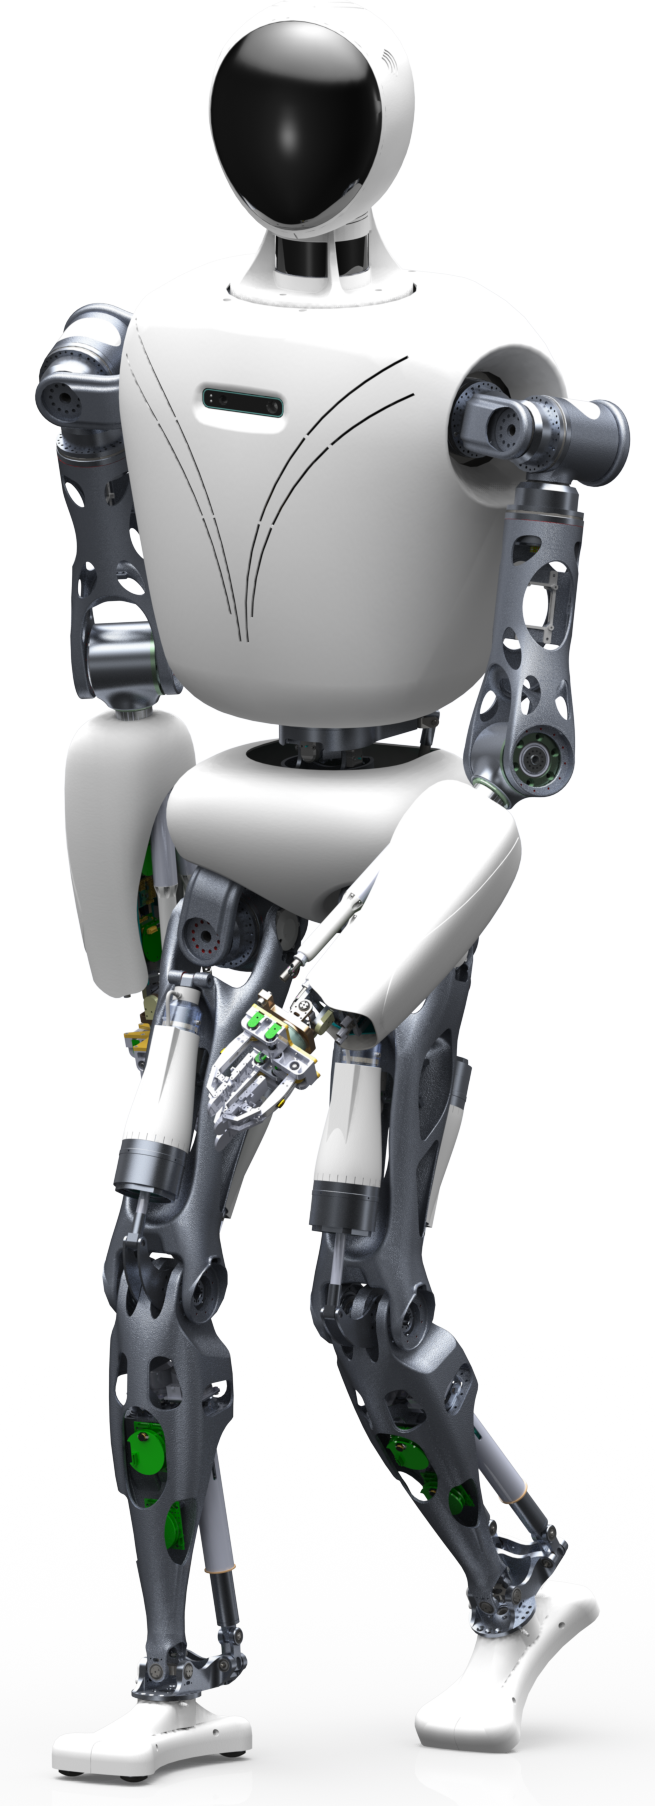
\includegraphics[width=.3\textwidth]{img/rh5_robot.png}
\caption{The recently presented RH5 is a lightweight and biologically inspired humanoid used as experimental platform within this thesis.}
\label{img:rh5_robot}
\end{figure} 


\section{Contribution and Structure}



